\documentclass[10pt, a4paper, twocolumn]{article}
\usepackage{geometry}
\geometry{left=0.5cm,right=0.5cm,top=0.5cm,bottom=0.5cm}
\linespread{0.5}
\usepackage{ctex}
\usepackage{graphicx}
\usepackage{amsthm}
\usepackage{amsmath}
\renewcommand{\vec}[1]{\boldsymbol{#1}}
\usepackage{amssymb}
\usepackage{booktabs}
\usepackage{hyperref}
\usepackage{multicol}
\setlength\columnsep{0.4cm}  % 设置两栏之间的间距为0.6cm
\columnseprule=1pt           % 实现插入分隔线,用于分栏

\usepackage{enumitem}

\newtheorem{definition}{定义}
\newtheorem{lemma}{引理}
\newtheorem{theorem}{定理}
\DeclareMathOperator{\Ima}{Im}%定义新符号
\DeclareMathOperator{\Rank}{rank}%定义求秩算子


\setlength{\floatsep}{2pt plus 2pt minus 2pt}
\setlength{\textfloatsep}{2pt plus 2pt minus 2pt}
\setlength{\intextsep}{2pt plus 2pt minus 2pt}


\begin{document}


\section{Time, Analysis, Vocabulary}
\begin{enumerate}[leftmargin = 12pt, topsep = 0pt, itemsep=0pt, partopsep = 0pt]
    \item Big $O$/$\omega$ Notation || Little $o$/$\omega$ Notation
    \item Amortized Analysis 均摊法:\\
        聚合分析:计算一组操作的平均耗时;\\
        势能分析:potential function $\Phi$ to evaluate current state; 每个操作的摊还代价=实际代价+引起的势能变化.
    \item a counterexample to prove low boundary.
    \item The problem is clearly in NP, as a $\dots$ can be served as a certificate. 
\end{enumerate}
\vspace{0.1cm}
\hrule
\section{Divide and Conquer}
\begin{enumerate}[leftmargin = 12pt, topsep = 0pt, itemsep=0pt, partopsep = 0pt]
    \item Karatsuba Algorithm for mulitiplication: \\one $n$-digit mul $\to$ three $\frac{n}{2}$-digit mul, $O(n^{\log_23})$.
    \item Merge Sort: 无序数列二分,有序子数列归并;双指针$O(m+n)$, $O(n\log n)$.
    \item Master Theorem: $T(n) = aT(n/b) + O(n^d)$
    \begin{figure}[htbp] %htbp
    \centering
    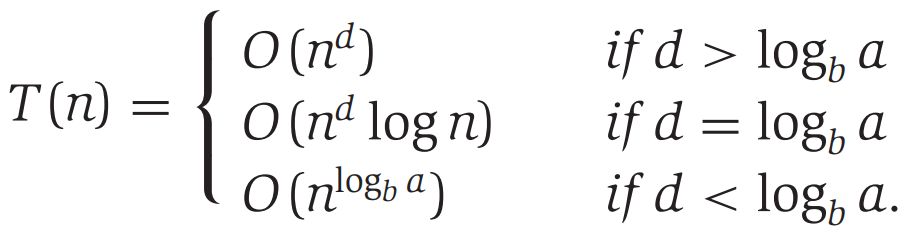
\includegraphics[scale=0.4]{pic/2_1.png}
    \end{figure}
    \vspace{-0.3cm}
    \item Counting Inversions: count while merging, $O(n\log n)$.
    \item Selection,找第几大/小: 随机算法$O(n)$\\
        Function $Select(S,k)$: Divide $O(n)$:
        \begin{itemize}[leftmargin = 12pt, topsep = 0pt, itemsep=0pt, partopsep = 0pt]
        \item pick an random value $v$ from $S$
        \item divide into three subsets: $L: x<v; M: x=v; R: x>v$
        \end{itemize}
        Recurse:
        \begin{itemize}[leftmargin = 12pt, topsep = 0pt, itemsep=0pt, partopsep = 0pt]
        \item If $k\leq |L|$, Select($L,k$); $|L|<k\leq |L|+|M|$, output $v$; $|L|+|M| < k$, Select($R, k-|L|+|M|$).
        \end{itemize}
        With 1/2 probability to reduce $T(n)$ to $T(3n/4)$, i.e. 2 rounds are expected. So $T(n) = T(3n/4) + O(n)\to O(n)$.
        \item Closet Pair: two-dimension points, find $\dots$, $O(n\log^2 n).$\\
        Function $ClosestPair(S)$: Divide $O(n\log n)$:
        \begin{itemize}[leftmargin = 12pt, topsep = 0pt, itemsep=0pt, partopsep = 0pt]
        \item Sort the points by x-coordinate
        \item Draw a vertical line $l$ so that each side has $n/2$ points
        \end{itemize}
        Recurse $2T(n/2)$:
        \begin{itemize}[leftmargin = 12pt, topsep = 0pt, itemsep=0pt, partopsep = 0pt]
        \item Find the closet pair in each side, distance $\delta_L,\delta_R$
        \end{itemize}
        Combine $O(n\log n)$:
        \begin{itemize}[leftmargin = 12pt, topsep = 0pt, itemsep=0pt, partopsep = 0pt]
        \item $\delta = min(\delta_L,\delta_R)$, $S^{'}$ be the points within $\delta$ from $l$
        \item Sort $S^{'}$ by the y-coordinate
        \item For each $a\in S^{'}$ check 7 $b\in S^{'}$ above $a$, find closest.
        \end{itemize}
        There are at most 4 points in a $\delta\times\delta$ square.
\end{enumerate}
\vspace{0.1cm}
\hrule
\section{Graph}
\begin{enumerate}[leftmargin = 12pt, topsep = 0pt, itemsep=0pt, partopsep = 0pt]
    \item Store: adjacency matrix, $O(|V|^2)$; adjacency list, $O(|V|+|E|)$.
    \item DFS, $O(|V|+|E|)$.\\
        Function $explore(v)$:
        \begin{itemize}[leftmargin = 12pt, topsep = 0pt, itemsep=0pt, partopsep = 0pt]
        \item $marked[v]\leftarrow true$
        \item for each $(u,v)\in E$: if $marked[u]=false$, $explore(u)$.
        \end{itemize}
        Function $dfs(G):$
        \begin{itemize}[leftmargin = 12pt, topsep = 0pt, itemsep=0pt, partopsep = 0pt]
        \item for each $v\in V$: if $marked[v]=false$, $explore(v)$.
        \end{itemize}
        On undirected graphs, DFS can: find connected components; detect cycles.
    \item Topological Order in DAG(有向无环) by DFS, $O(|V|+|E|)$.\\
        Function $explore(v)$:
        \begin{itemize}[leftmargin = 12pt, topsep = 0pt, itemsep=0pt, partopsep = 0pt]
        \item $start[v]\leftarrow time$; $time++$
        \item $marked[v]\leftarrow true$
        \item for each $(u,v)\in E$: if $marked[u]=false$, $explore(u)$.
        \end{itemize}
        Function $dfs(G):$
        \begin{itemize}[leftmargin = 12pt, topsep = 0pt, itemsep=0pt, partopsep = 0pt]
        \item for each $v\in V$: if $marked[v]=false$, $explore(v)$
        \item $finish[v]\leftarrow time$; $time++$.
        \end{itemize}
    \item Strong Connected Component(SCC) by DFS, $O(|V|+|E|)$.
        Find the vertex in the head SCC in the reverse graph.
        \begin{itemize}[leftmargin = 12pt, topsep = 0pt, itemsep=0pt, partopsep = 0pt]
        \item DFS on $G^R$(reversed $G$) and maintain a sorted list by the finish time
        \item DFS $G$ by the descending order of the finish time, and each $explore()$ forms a SCC.
        \end{itemize}
    \item BFS, $O(|V|+|E|)$.
        \begin{table}[htbp]
    	\centering
    	\begin{tabular}{ccc}
    		\hline\hline\noalign{\smallskip}	
    		 & DFS & BFS  \\
    		\noalign{\smallskip}\hline\noalign{\smallskip}
    		Detecting Cycles & yes & no \\
    		Topological Ordering & yes & no \\
    		Finding CCs & yes & yes \\
    		Finding SCCs & yes & no \\
    		Shortest path & no & yes \\
    		\noalign{\smallskip}\hline
    	\end{tabular}
        \end{table}
    \item Dijkstra Algorithm for shortest path(weighted, positive), time dependents on the priority queue.\\
        每次从[未求出最短路径的点]中取出距离起点最小路径的点,以这个点为桥梁刷新[未求出最短路径的点]的距离。\\
        Function $Dijkstra(G=(V,E),s)$: Initialize:
        \begin{itemize}[leftmargin = 12pt, topsep = 0pt, itemsep=0pt, partopsep = 0pt]
        \item $T\leftarrow \{s\}$; $tdist[v]\leftarrow w(s,v)$, $pre[v]\leftarrow s$ for all $(s,v)\in E$
        \end{itemize}
        Explore, $|V|$ rounds:
        \begin{itemize}[leftmargin = 12pt, topsep = 0pt, itemsep=0pt, partopsep = 0pt]
        \item Find $v\notin T$ with smallest $tdist[v]$; $T\leftarrow T+\{v\}$
        \end{itemize}
        Update $tdist[u]$, $|E|$ rounds:
        \begin{itemize}[leftmargin = 12pt, topsep = 0pt, itemsep=0pt, partopsep = 0pt]
        \item $tdist[u]=min\{tdist[u], tdist[v]+w(v,u)\}$ for all $(u,v)\in E$
        \item If $tdist[u]$ is updated, then $pre[u]\leftarrow v$.
        \end{itemize}
        Find Min: $|V|$ rounds; Update $|E|$ rounds;\\
        \begin{table}[htbp]
    	\centering
    	\begin{tabular}{ccccc}
    		\hline\hline\noalign{\smallskip}	
    		 & Pop Min & Insert & Update & Merge  \\
    		\noalign{\smallskip}\hline\noalign{\smallskip}
    		Binary Heap & $O(\log n)$ & $O(\log n)$ & $O(\log n)$ & $O(n)$ \\
    		d-nary Heap & $O(d\log_d n)$ & $O(\log_d n)$ & $O(\log_d n)$ & $O(n)$ \\
    		Binomial Heap & $O(\log n)$ & $O(1)$ & $O(\log n)$ & $O(\log n)$ \\
    		Fibonacci & $O(\log n)$ & $O(1)$ & $O(1)$ & $O(1)$\\
    		\noalign{\smallskip}\hline
    	\end{tabular}
        \end{table}
        the $O(1)$ update of Fibonacci is only for dereasing. 
    \item Bellman-Ford for shortest path(negative), $O(|V||E|)$.\\
    对所有的边进行$n-1$轮松弛操作。\\
    Lemma 1: After $k$ rounds, $dist(v)$ is the shortest distance of all $k$-edge-path (paths with at most $k$ edges).\\
    Lemma 2: The shortest distance of all $|V|$-edge-path can not be shorter than the shortest distance of all $(|V|-1)$-edge-path unless there is a Negative Cycle.\\
    Algorithm: Run $|V|$ rounds updating, if distance become shorter in the $|V|$-th round, output negative cycle, otherwise output distance.
\end{enumerate}
\vspace{0.1cm}
\hrule
\section{Greedy}
\begin{enumerate}[leftmargin = 12pt, topsep = 0pt, itemsep=0pt, partopsep = 0pt]
    \item Prim Algorithm for Minimum Spanning Tree, Dijkstra's        growing idea, $O(|E|+|V|\log|V|)$ if Fibonacci Heap.\\
        每次选出一个离[生成树]距离最小的点去加入[生成树]。\\
        Negative weight no matter because length of path is sure.\\
        Function $Prim(G=(V,E))$: Initialize:
        \begin{itemize}[leftmargin = 12pt, topsep = 0pt, itemsep=0pt, partopsep = 0pt]
        \item $T\leftarrow \{\},S\leftarrow \{s\}$
        \item $cost[s]=0, cost[v]\leftarrow \infty$ for all $v$ other than s
        \item $cost[v]\leftarrow w(s,v), pre[v]=s$ for all $(s,v)\in E$
        \end{itemize}
        Explore:
        \begin{itemize}[leftmargin = 12pt, topsep = 0pt, itemsep=0pt, partopsep = 0pt]
        \item Find $v\in S$ with smallest $cost[v]$
        \item $S\leftarrow S_\{v\}$; $T\leftarrow T+\{(pre[v],v)\}$
        \end{itemize}
        Update $cost[u]$:
        \begin{itemize}[leftmargin = 12pt, topsep = 0pt, itemsep=0pt, partopsep = 0pt]
        \item $cost[u]=min\{cost[u],w(v,u)\}$ for all $(v,u)\in E$
        \item If $cost[u]$ is updated, then $pre[u]=v$.
        \end{itemize}
    \item Kruskal Algorithm for MST, $O(|E|\log|V|)$ if union-find       set.\\
        从小到大选边,如果不和已选择的边构成环路,选择它组成最小生成树(林)。\\
        Function $Kruskal(G=(V,E))$:
        \begin{itemize}[leftmargin = 12pt, topsep = 0pt, itemsep=0pt, partopsep = 0pt]
        \item Sort the edge set $E$ to ascending order
        \item For each $e\in E$ in ascending order: If $e$ does not create a cycle, then choose it \\
        i.e. If $group(u)!=group(v)$:\\ choose $(u,v)$, $union(group(u),group(v))$.
        \end{itemize}
        $O(|E|\log|E|)=O(|E|\log|V|)$ for sorting; $2|E|$ round: check group; $|V|$ round: union group.\\
        Union-find Set: Find: $O(\log n)$; Union: $O(1)$.
    \item Greedy Prove: the local greedy choice do not ruin out OPT.\\
        Induction:
        \begin{itemize}[leftmargin = 12pt, topsep = 0pt, itemsep=0pt, partopsep = 0pt]
        \item Base step: $\emptyset$ is in an OPT
        \item Hypothesis: the selected $k-1$ activities are in an $OPT$
        \item Induction: After adding the $k$-th activity, we are still in an OPT
        \item Conclusion: After adding the last activity, it is in an OPT. Nothing can be added, so it is OPT.
        \end{itemize}
    \item Huffman Encoding for compression, $O(n\log n)$.\\
        Sort the characters by their appearance.\\
        Repeat $n$ rounds:
        \begin{itemize}[leftmargin = 12pt, topsep = 0pt, itemsep=0pt, partopsep = 0pt]
        \item Find two minimized appearance elements
        \item Delete two minimized element
        \item Insert a super node into the list.
        \end{itemize}
\end{enumerate}
\vspace{0.1cm}
\hrule
\section{Dynamic Programming}
In dynamic programming we construct a DAG. Its nodes are the sub-problems we define, and its edges are the dependencies between the sub-problems.
\begin{enumerate}[leftmargin = 12pt, topsep = 0pt, itemsep=0pt, partopsep = 0pt]
    \item Number of Sub-problem:
        \begin{itemize}[leftmargin = 12pt, topsep = 0pt, itemsep=0pt, partopsep = 0pt]
        \item Input $x_1,x_2,\dots,x_n$, sub $x_1,x_2,\dots,x_i$: linear
        \item Input $x_1,x_2,\dots,x_n$ and $y_1,y_2,\dots,y_m$, sub $x_1,x_2,\dots,x_i$ and $y_1,y_2,\dots,y_j$: $O(mn)$
        \item Input $x_1,x_2,\dots,x_n$, sub $x_i,x_{i+1},\dots,x_j$: $O(n^2)$.
        \end{itemize}
    \item Shortest Path in DAG\\
        \begin{equation}
        	dist(t) = min \begin{cases}
        	dist(v_1)+w(v_1,t)\\
        	dist(v_2)+w(v_2,t)\\
        	\dots
        	\end{cases}
        \nonumber 
        \end{equation}
    \item Longest Increasing Sub-sequence, $O(n^2)$.\\
        Sub-problems: $LIS[k]$ the longest increasing sub-sequence ended by $a_k$.\\
        Function $LIS(n)$:
        \begin{itemize}[leftmargin = 12pt, topsep = 0pt, itemsep=0pt, partopsep = 0pt]
        \item $lis[0]\leftarrow 0$
        \item for $i=1\to n$: $lis[i]=max_{a_j<a_i,j<i}\{lis[j]+1\}$
        \item return $max_{1\leq i\leq n}lis[i]$.
        \end{itemize}
    \item Edit Distance, the steps of Insertion/Deletion/Replacement     to change one string to another, $O(mn)$.\\
        Sub-problems: $E(i,j)$ distance between $X[1\dots i], Y[1,\dots, j]$\\
        \begin{equation}
        	E(i,j) = min \begin{cases}
        	1+E(i-1,j)\\
        	1+E(i,j-1)\\
        	diff(i,j)+E(i-1,j-1)
        	\end{cases}
        \nonumber 
        \end{equation}
    \item Knapsack Problems, for given $n$ items with cost $c_i$ and     value $v_i$, and a capacity $W$, select a subset of items        with total cost at most $W$, to maximize the total value.        $O(nW)$.\\
        Sub-problems: $f[i,w]$ the maximum value we can get by using the first $i$ items and with $w$ budget.\\
        Buy single: $f[i,w] = max\{ f[i-1,w], f[i-1,w-c_i]+v_i\}$.\\
        Buy some: $f[i,w] = max\{ f[i-1,w], f[i,w-c_i]+v_i\}$.\\
        Function: $knapsack(n)$:
        \begin{itemize}[leftmargin = 12pt, topsep = 0pt, itemsep=0pt, partopsep = 0pt]
        \item $lis[0]\leftarrow 0$
        \item $f[0,0]=f[0,1]=\dots f[0,W]=0$
        \item $f[0,0]=f[1,0]=\dots f[n,0]=0$
        \item for $w=0\to W$: for $i=1\to n$: \\
        $f[i,w] = max\{ f[i-1,w], f[i,w-c_i]+v_i\}$
        \item return $f[n,W]$.
        \end{itemize}
        Assume that the input size $=N$, $W=2^N$ by using $N$ bits, $O(nW)=O(N2^N)$.
    \item Largest Number in $k$ Consecutive Numbers, given a sequence     of numbers, output the largest number in every $k$               consecutive numbers. $O(n)$.\\
        Sub-problems: $large[i]$ the largest number from $a_{i-k+1}$ to $a_i$.\\
        $PLL[i]$ the potential largest list for $a_{i-k+1}$ to $a_i$. 更新:去掉又老又菜的,加入新的,维持递减。\\
        Updating Priority Queue: \\
        Function $updating(a[1,\dots,n],i,k,PLL)$:
        \begin{itemize}[leftmargin = 12pt, topsep = 0pt, itemsep=0pt, partopsep = 0pt]
        \item If $PLL.front.index\leq i-k$: $PopFront(PLL)$
        \item while $PLL.back.value \leq a[i]$: $Popback(PLL)$
        \item $Pushback(PLL,(index=i,value=a[i])$.
        \end{itemize}
        Largest Number in range $k$:\\
        Function $largest(a[1.\dots,n],k)$:
        \begin{itemize}[leftmargin = 12pt, topsep = 0pt, itemsep=0pt, partopsep = 0pt]
        \item $PLL = NULL$
        \item for $i=1\to n$: $updating(a,i,k,PLL)$, output $PLL.front$.
        \end{itemize}
        Each number charged once when popped in and once, $O(n)$.
    \item Longest Increasing Sequence with Priority Queue, $O(n\log n)$.\\
        Define Potential prefix: the set of $a_j$ that is possible to be the best prefix of future numbers.\\
        $sm[len]$ the smallest ended number for a increasing sub-sequence with length $len$.\\
        The DP Algorithm:
        \begin{itemize}[leftmargin = 12pt, topsep = 0pt, itemsep=0pt, partopsep = 0pt]
        \item initialize $sm[0]\leftarrow 0$ with $a_i$ by Binary Search
        \item output the largest $len$ such that $sm[len]$ is updated.
        \end{itemize}
    \item Product of Sets, given $n$ set $L_1,\dots, L_n$, output the     minimum number of operations to calculate $L_1\times \dots       L_n$. $O(n^3)$.\\
        Sub-problems: $c(i,j)$ is the cost for calculating $L_1\times L_j$.\\
        $c(i,j)=m_i m_{i+1} \dots m_j + min_{i\leq k<j}\{ c(i,k) + c(k+1,j) \}$.\\
        $n^2$ sub-problems and $n$ iterations to calculate each. $O(n^3)$.
    \item Maximize Independent Set on Trees, $O(n)$.\\
        Sub-problems: $f[v]$ the maximized size of independent set of the sub-tree rooted at $v$.\\
        $f[v]= max\{ \sum_{u\in children(v)}f[u], \sum_{u\in grandchildren(v)}f[u] + 1 \}$.\\
        Each of its children and its grandchildren cost one. So every vertex pays for parent and grandparent. $O(n)$.
\end{enumerate}
\vspace{0.1cm}
\hrule
\section{Max-Flow and Linear Programming}
\vspace{-1cm}
\begin{align*}
	\mbox{max } & \sum_{(s,v)\in E}f(s,v) \\
	\mbox{s.t. } & 0\leq f(u,v) \leq c_{uv} \mbox{ for } (u,v)\in E\\
	 & \sum_{(u,v)\in E} = \sum_{(v,w)\in E}f(v,w) \mbox{ for all } v \in V/\{s,t\}
\end{align*}
Residual network $G^f=(V,E^f)$, which has two types of edges, with residual capacities $c^f$: 剩余流量和后悔流量
\begin{equation}
        	\begin{cases}
        	c_{uv} - f_{uv}, & \text{ if } (u,v)\in E \text{ and } f_{uv} < c_{uv}\\
        	f_{vu}, & \text{ if } (v,u)\in E \text{ and } f_{vu} > c_{uv}
        	\end{cases}
        \nonumber 
        \end{equation}
\begin{enumerate}[leftmargin = 12pt, topsep = 0pt, itemsep=0pt, partopsep = 0pt]
    \item Ford-Fulkerson Algorithm, $O(|E|\cdot f_{max})$:
        \begin{itemize}[leftmargin = 12pt, topsep = 0pt, itemsep=0pt, partopsep = 0pt]
        \item Initialize an empty flow $f$ and the corresponding residual flow $G^f$
        \item while until there is no $s-t$ path on $Gf$:\\
            find a path on $G^f$\\
            push maximum amount of flow on $G^f$, update $f,G^f$.
        \end{itemize}
        If there are both $(u,v),(v,u)\in E$, add a middle node to modify the graph.\\
        该算法在无理数情况下无法保证终止,在有理数/整数情况下无法保证多项式时间复杂度。\\
        If all capacities are integers, each iteration requires $O(|E|)$, there are at most $f_{max}$ iterations. $O(|E|\cdot f_{max})$.\\
    \item Integral Theorem: If each $c(e)$ is an integer, then the       value of the maximum flow $f_{max}$ is an integral.              应用到整数问题需要说明。
    \item Max-Flow-Min-Cut Theorem: The value of the maximum flow is     exactly the value of the minimum cut $max_f v(f) =               min_{L,R}c(L,R)$.\\
    \item Edmonds-Karp Algorithm for Max-Flow, $O(|V|\cdot |E|^2)$.\\
        通过每次用BFS寻找$s-t$ path的方式来执行Ford-Fulkerson,保证了residual network当中每个点离s距离的单调性,从而实现多项式时间复杂度。\\
        BFS maintains the distance(num of edges). And $dist(u)$ in $G^f$ is non-decreasing.\\
        A edge $(u,v)$ is critical if the amount of flow pushed along $p$ is $c^{f_i}(u,v)$.\\
        \textbf{Algorithm:}
        \begin{itemize}[leftmargin = 12pt, topsep = 0pt, itemsep=0pt, partopsep = 0pt]
        \item initialize $f$ such that $\forall e\in E$: $f(e)=0$; initialize $G^f\leftarrow G$
        \item while there is a $s-t$ path on $G^f$:\\
            find such a path $p$ by BFS\\
            find an edge $e\in p$ with minimum capacity $b_i$\\
            update $f$ that pushes $b$ units of flow along $p_i$\\
            update $G^f$
        \item return $f$.
        \end{itemize}
        \textbf{between two "critical":}
        \begin{itemize}[leftmargin = 12pt, topsep = 0pt, itemsep=0pt, partopsep = 0pt]
        \item $i\mbox{th iterations: }s \dots u \to v\dots t$: $dist^i(v)=dist^i(u)+1$
        \item $i+1\mbox{th iterations: }s \dots u \leftarrow v\dots t$
        \item $\dots$
        \item before $u\to v$ reappears: $i+j\mbox{th iterations: } s \dots v \to u \dots t$: $dist^{i+j}(u)=dist^{i+j}(v)+1$
        \end{itemize}
        \textbf{TIME}
        \begin{itemize}[leftmargin = 12pt, topsep = 0pt, itemsep=0pt, partopsep = 0pt]
        \item $dist(u)$ increases by 2 between 2 "critical";
        \item $dist(u)$ can only be $0,1,2,\dots,|V|,\infty$ and never decreases;
        \item at least one edge becomes "critical" in one iteration;
        \item each edge becomes "critical" at most $O(|V|)$ times;
        \item iterations $O(|E|\cdot|V|)$, time complexity $O(|V|\cdot|E|^2)$.
        \end{itemize}
    \item Dinic's Algorithm for Max-Flow, $O(|V|^2\cdot|E|)$.\\
        try to make some dist strictly increasing.\\
        Level Graph: 
        \begin{itemize}[leftmargin = 12pt, topsep = 0pt, itemsep=0pt, partopsep = 0pt]
        \item Vertices at level $i$ are at distance $i$
        \item Only edges go from a level to the next level are kept
        \item Can be done in $O(|E|)$ time using a similar idea to BFS
        \end{itemize}
        Block flow:
        \begin{itemize}[leftmargin = 12pt, topsep = 0pt, itemsep=0pt, partopsep = 0pt]
        \item Push flow on multiple $s-t$ paths
        \item Each $s-t$ path must contain a critical edge
        \end{itemize}
        \textbf{Algorithm:}
        \begin{itemize}[leftmargin = 12pt, topsep = 0pt, itemsep=0pt, partopsep = 0pt]
        \item Initialize $f$ to be the empty flow and $G^f=G$
        \item do until $dist(t) = \infty$:\\
            Construct the level graph $G^f_L$\\
            Find a blocking flow on $G^f_L$\\
            Update $f$ and $G^f$\\
        \end{itemize}
        \vspace{-0.5cm}
        \textbf{Find a block flow in a level graph:}
        \begin{itemize}[leftmargin = 12pt, topsep = 0pt, itemsep=0pt, partopsep = 0pt]
        \item do until no path from $s$ to $t$:\\
            Run a frontward DFS\\
            If end up at $t$: update $f$ and remove the critical edge\\
            IF end up at vertex $v$: remove all the incoming edges of $v$
        \item At least one edge is removed after each search. Each search takes $O(|V|)$. Time complexity $O(|V|\cdot|E|)$.
        \end{itemize}
        \textbf{How many iteration:}
        \begin{itemize}[leftmargin = 12pt, topsep = 0pt, itemsep=0pt, partopsep = 0pt]
        \item In $G^{f_i}_L$, every $s-t$ path has length $dist^i(t)$
        \item Still, $dist(u)$ is non-decreasing.
        \item Proving $dist^{i+1}(t)>dist^i(t)$ by contradiction $dist^{i+1}(t)=dist^i(t)$:\\
            All edges appear in $G^{f_i}_L$: path contains no critical edge.\\
            $(u,v)$ not in $G^{f_i}_L$: $(u,v)$ is a backward or same level edge.
        \item $dist(t)$ is increased in each iteration so $O(|V|)$ iterations.
        \end{itemize}
    \item Maximum Bipartite Matching\\
        Hall's Marriage Theorem: There exists a matching of size $|A|$ iff $|S|\leq |Neighbor(S)|$ for every $S\subseteq A$.\\
        A graph is regular if all the vertices have the same degree.  A match is perfect if all vertices are matched. Regular graph has perfect matching.
    \item Hopcroft–Karp–Karzanov Algorithm for maximum bipartite         matching, Special case of Dinic's, $O(|E|\cdot\sqrt{|V|})$.\\
        \textbf{Find a blocking flow in a level graph takes $O(|E|)$:}
        \begin{itemize}[leftmargin = 12pt, topsep = 0pt, itemsep=0pt, partopsep = 0pt]
        \item do until no path from $s$ to $t$:\\
            DFS from $s$.\\
            End up at $t$: delete this path, start over from $s$.\\
            Have to go backward or blocked, delete the edge just travelled.
        \end{itemize}
        Each edge is visted at most once, $O(|E|)$.
        \textbf{Iterations at most $2\sqrt{|V|}$:}
        \begin{itemize}[leftmargin = 12pt, topsep = 0pt, itemsep=0pt, partopsep = 0pt]
        \item If algotithm ends within $\sqrt{|V|}$ iterations, done.
        \item Otherwise, let $f$ be the flow after $\sqrt{|V|}$ iterations:\\
            Dinic's proves $dist^{G^f}(s,t)\geq \sqrt{|V|}$; \\
            By induction, $\forall v\in V- \{s,t\}$, either in-degree or ou-degree is 1.
            So there exists a maximum integral flow $f^{'}$ consisting of
            vertex-disjoint paths with flow 1.
            Hence, there are at most $\frac{|V|}{\sqrt{|V|}}=\sqrt{|V|}$ paths in $f^{'}$.
        \end{itemize}
        Total number of iterations: $2\sqrt{|V|}$.
    \item LP-Relaxation\\
        Standard Form LP: Maximization as objective with $\leq$ constraints and non-negative variables.\\
        Interger Linear Program(ILP): each variable is an integer.
    \item LP Duality\\
        max/min the linear combination of constraints of the primal problem, the coefficients of primal problem become the boundary. LP has strong duality theorem.
    \item Applications of LP-Duality\\
        The dual program of max-flow is the fractional version of min-cut. It always have integral optimum, so max-flow = min-cut.\\
        \textbf{When LP has optimal integral solution?}\\
        simplex method $\to$ all vertices are integral.\\
        A matrix $A$ is totally unimodular if every square submatrix has determinant $0,1$ or $-1$.
        \begin{itemize}[leftmargin = 12pt, topsep = 0pt, itemsep=0pt, partopsep = 0pt]
        \item If $A\in \mathbb{R}^{m\times n}$ is totally unimodular     and $b$ is an integer vector, then the polytope             $p=\{x:Ax\leq b\}$ has integer vertices.
        \item LP $Ax\leq b$, if $A$ is unimodular, OPT is integral when $b$ is integral.
        \item $A$ is totally unimodular, then so are $A^T,[I A],[AI],[I A]^T,[AI]^T$.v.v.
        \end{itemize}
        \textbf{Use strong duality theorem to prove some theorems: }
        \begin{itemize}[leftmargin = 12pt, topsep = 0pt, itemsep=0pt, partopsep = 0pt]
        \item write down the primal and dual LPs.
        \item Justify that the primal and dual LPs describe the corresponding problems.
        \item If the problem is discrete, prove that the corresponding LP always gives integral solution.
        \item Apply strong duality theorem.
        \end{itemize}
\end{enumerate}
\vspace{0.1cm}
\hrule
\section{NP}
NP-complete: SAT/Vertex Cover/Independent Set/Subset Sum/Hamiltonian Path、cycle\\
The problem is clearly in NP, as $\dots$ can be served as a certificate. To show it is NP-complete, we present a reduction from $\dots$. Given a$\dots$ instance $\dots$, we construct an instance $\dots$ for this problem.\\
If the $\dots$ instance is a yes instance, $\dots$\\

% 	\fbox{
% 	\parbox{9cm}{}
% 	}

%\begin{figure}[ht] %htbp
%\centering
%\includegraphics[scale=0.6]{ai.png}
%\caption{this is a figure demo}
%\label{fig:label}
%\end{figure}

% \begin{equation}\label{fft}
% 	F(\omega) = \mathcal{F}[f(t)] = \int_{-\infty}^{\infty} f(t)e^{-i\omega t} \mathrm{d}t
% \end{equation}

% \section{损失函数和最优化}

% \begin{enumerate}
%     \item one
%     \item two
%     \item ...
% \end{enumerate}

\end{document}
